\documentclass[ignorenonframetext,]{beamer}
\setbeamertemplate{caption}[numbered]
\setbeamertemplate{caption label separator}{:}
\setbeamercolor{caption name}{fg=normal text.fg}
\usepackage{amssymb,amsmath}
\usepackage{ifxetex,ifluatex}
\usepackage{fixltx2e} % provides \textsubscript
\usepackage{lmodern}
\ifxetex
  \usepackage{fontspec,xltxtra,xunicode}
  \defaultfontfeatures{Mapping=tex-text,Scale=MatchLowercase}
  \newcommand{\euro}{€}
\else
  \ifluatex
    \usepackage{fontspec}
    \defaultfontfeatures{Mapping=tex-text,Scale=MatchLowercase}
    \newcommand{\euro}{€}
  \else
    \usepackage[T1]{fontenc}
    \usepackage[utf8]{inputenc}
      \fi
\fi
% use upquote if available, for straight quotes in verbatim environments
\IfFileExists{upquote.sty}{\usepackage{upquote}}{}
% use microtype if available
\IfFileExists{microtype.sty}{\usepackage{microtype}}{}
\usepackage{url}
\usepackage{graphicx}
\makeatletter
\def\maxwidth{\ifdim\Gin@nat@width>\linewidth\linewidth\else\Gin@nat@width\fi}
\def\maxheight{\ifdim\Gin@nat@height>\textheight0.8\textheight\else\Gin@nat@height\fi}
\makeatother
% Scale images if necessary, so that they will not overflow the page
% margins by default, and it is still possible to overwrite the defaults
% using explicit options in \includegraphics[width, height, ...]{}
\setkeys{Gin}{width=\maxwidth,height=\maxheight,keepaspectratio}

% Comment these out if you don't want a slide with just the
% part/section/subsection/subsubsection title:
\AtBeginPart{
  \let\insertpartnumber\relax
  \let\partname\relax
  \frame{\partpage}
}
\AtBeginSection{
  \let\insertsectionnumber\relax
  \let\sectionname\relax
  \frame{\sectionpage}
}
\AtBeginSubsection{
  \let\insertsubsectionnumber\relax
  \let\subsectionname\relax
  \frame{\subsectionpage}
}

\setlength{\parindent}{0pt}
\setlength{\parskip}{6pt plus 2pt minus 1pt}
\setlength{\emergencystretch}{3em}  % prevent overfull lines
\setcounter{secnumdepth}{0}

\title{Adding nucleo-olivary inhibition to a bottom-up computational model of
the vestibulo-ocular reflex to control gaze stabilization}
\author{Xavier Duran, supervised by Ivan Herreros and Paul Verschure}
\date{March 25, 2015}

\begin{document}
\frame{\titlepage}

\begin{frame}{Trade-offs in avoidance actions}

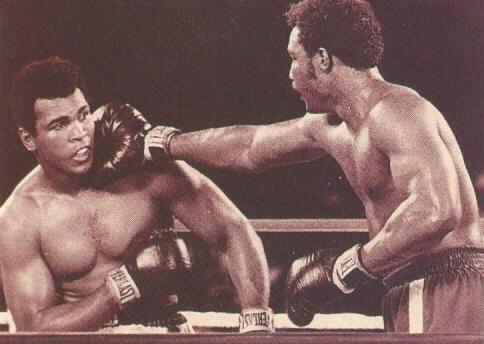
\includegraphics{images/ali.png}\footnote{\url{http://bit.ly/1OyIoEI}}

\end{frame}

\begin{frame}{Optimization of aversive reflexes}

\begin{itemize}
\itemsep1pt\parskip0pt\parsep0pt
\item
  Avoid aversive stimuli with minimum necessary effort
\item
  How we behave carries a cost: What we fail to prevent + preventing
  action itself
\item
  The ideal actions are those that minimize the overall cost
\end{itemize}

(Brandi, Herreros, and Verschure 2014)

\end{frame}

\begin{frame}{Nucleo-olivary inhibition (NOI)}

\begin{columns}[T]
\begin{column}[T]{5cm}
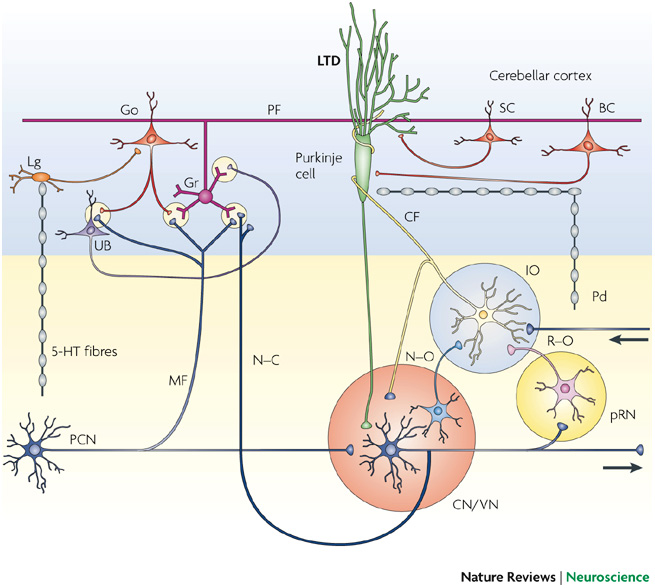
\includegraphics[]{images/nrn2332-f3.jpg}
\end{column}
\begin{column}[T]{5cm} % each column can also be its own environment
\begin{itemize}
\item Cost-optimization
\item Error-based learning
\item Acquired conditioned responses are extinguished once they become no longer necessary
\item The gain of the NOI is what determines the amplitude of the response on adaptive reflexes
\end{itemize}
\end{column}
\end{columns}

\footnote{\url{http://bit.ly/1AVg1qX}}

(Herreros and Verschure 2013)

\end{frame}

\begin{frame}{Eye-blink reflex conditioning}

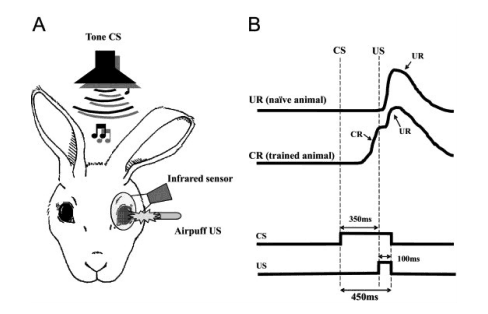
\includegraphics{images/eyeblink.png}

\footnote{\url{http://bit.ly/1CXvsoK}}

\end{frame}

\begin{frame}{NOI on eye-blink reflex}

\begin{itemize}
\itemsep1pt\parskip0pt\parsep0pt
\item
  Perceiving an air-puff in the unprotected cornea has a cost
\item
  Two types of costs

  \begin{itemize}
  \itemsep1pt\parskip0pt\parsep0pt
  \item
    Failing to avoid: error-based learning
  \item
    Avoiding when not necessary
  \end{itemize}
\item
  Extinction of unnecessary conditioned responses
\end{itemize}

(Herreros and Verschure 2013)

\end{frame}

\begin{frame}{Vestibulo-ocular reflex (VOR)}

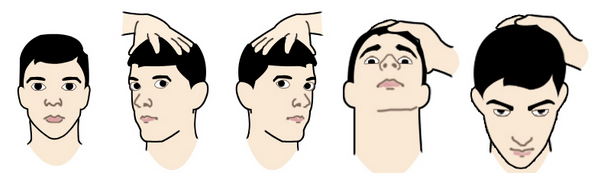
\includegraphics{images/vor.png}\footnote{\url{http://bit.ly/19GjJOA}}

This reflex functions to \textbf{stabilize images} on the retinas during
\textbf{head movement} by producing \textbf{eye movements} in the
direction opposite to head movement, thus preserving the image on the
center of the visual field.

\end{frame}

\begin{frame}{Vestibulo-ocular reflex (VOR) adaptation}

\begin{columns}[T]
\begin{column}[T]{5cm}
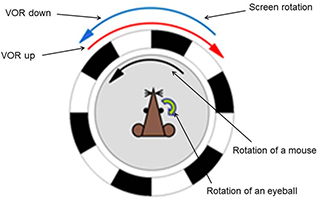
\includegraphics[]{images/13.jpg}
\end{column}
\begin{column}[T]{5cm} % each column can also be its own environment
\begin{itemize}
\item VOR adaptation is one of the most studied cerebellar dependent motor learning tasks
\item It is used to provide insight about the connections and the coding of the circuitry of the cerebellum
\end{itemize}
\end{column}
\end{columns}

\footnote{\url{http://bit.ly/1Ox3Qd6}}

\end{frame}

\begin{frame}{Problem statement}

\begin{quote}
Computational models of the vestibulo-ocular reflex don't take into
account the role of the nucleo-olivary inhibition
\end{quote}

\end{frame}

\begin{frame}{Research question}

\begin{quote}
What's the role of the nucleo-olivary inhibition in the vestibulo-ocular
reflex?
\end{quote}

\begin{block}{Fingerprints}

\begin{itemize}
\itemsep1pt\parskip0pt\parsep0pt
\item
  NOI has a role in the eye-blink reflex
\item
  There is extinction of the adaptive response in the absence of
  peripheral error
\item
  VOR adaptation has a non-perfect performance, with a residual error
  proportional to the amount of cerebellar action required
\end{itemize}

(Herreros and Verschure 2013)

\end{block}

\end{frame}

\begin{frame}{Hypothesis}

\begin{quote}
Adding nucleo-olivary inhibition on a detailed bottom-up state of the
art vestibulo-ocular reflex computational model would offer a more
parsimonious explanation of the experimental behavior of the reflex.
\end{quote}

\end{frame}

\begin{frame}{Computational models of the VOR}

Models of the cerebellar microcircuit

\begin{itemize}
\itemsep1pt\parskip0pt\parsep0pt
\item
  Marr-Albus-Ito classical models
\item
  Plasticity on the brainstem
\item
  A detailed bottom-up model
\end{itemize}

\end{frame}

\begin{frame}{Cerebellar cortex}

\begin{columns}[T]
\begin{column}[T]{5cm}
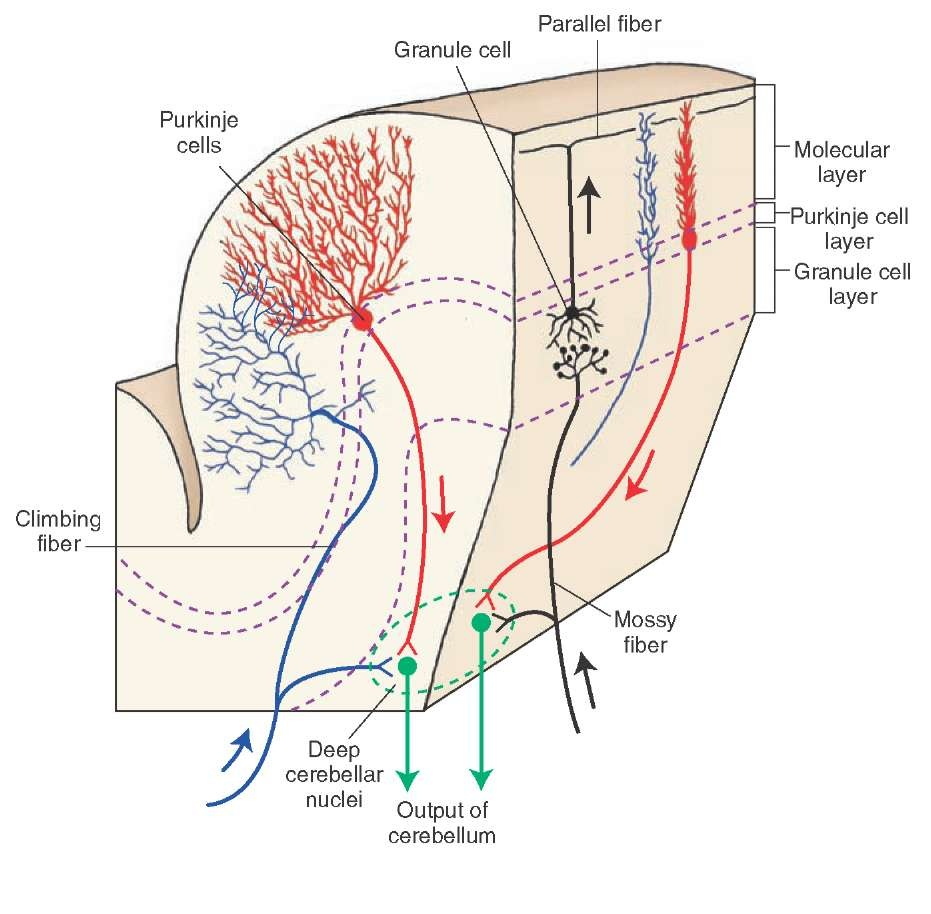
\includegraphics[height=3cm]{images/tmp15F112.jpg}
\end{column}
\begin{column}[T]{5cm} % each column can also be its own environment
\begin{itemize}
\item Uniform structure throughout the cerebellum
\item Composed of repeated modules or microzones
\item Same cell types and connectivity
\item Functional units
\item Different inputs, different targets
\item Cerebellar algorithm
\end{itemize}
\end{column}
\end{columns}

\footnote{\url{http://bit.ly/1CioLvp}}

\end{frame}

\begin{frame}{Marr-Albus-Ito classical models}

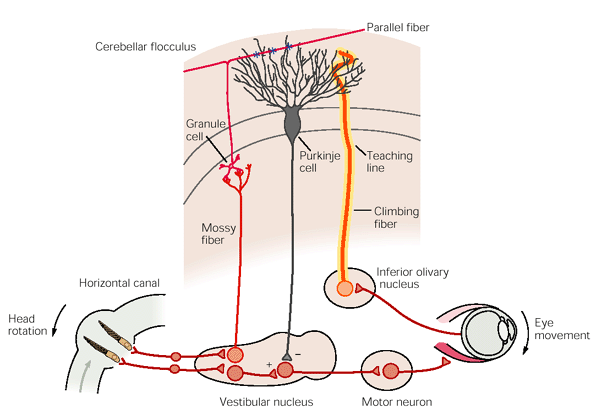
\includegraphics{images/ito.png}\footnote{\url{http://bit.ly/1ED2SEc}}

(Ito 2006)

\end{frame}

\begin{frame}{Plasticity on the brainstem}

\begin{itemize}
\itemsep1pt\parskip0pt\parsep0pt
\item
  Plasticity in both cerebellar cortex and the brainstem
\item
  Cerebellar cortex for quick adaptation
\item
  Brainstem as long-term memory
\item
  Brainstem learns a simple gain
\end{itemize}

(Ke, Guo, and Raymond 2009)

\end{frame}

\begin{frame}{A detailed bottom-up model}

This computational model is made bottom-up from physiological and
behavioral observations.

\begin{itemize}
\itemsep1pt\parskip0pt\parsep0pt
\item
  Plasticity on the cerebellar cortex
\item
  Plasticity on the brainstem
\item
  Delayed error signal
\item
  White noise on the signals
\item
  Contribution of interneurons
\end{itemize}

(Clopath et al. 2014)

\end{frame}

\begin{frame}{Methods}

\begin{itemize}
\itemsep1pt\parskip0pt\parsep0pt
\item
  Implementation of the detailed model (Clopath et al. 2014) of the VOR
\item
  Reproduction of the results of the paper
\item
  Add the NOI to the detailed model
\item
  Simulation of adaptation, extinction and readaptation of the VOR
\end{itemize}

\end{frame}

\begin{frame}{Experimental setup}

\begin{columns}[T] % contents are top vertically aligned
\begin{column}[T]{5cm} % alternative top-align that's better for graphics
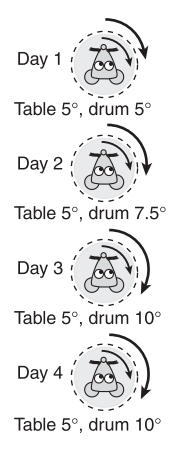
\includegraphics[height=3cm]{images/vvor.png}
\end{column}
\begin{column}[T]{5cm} % each column can also be its own environment
\begin{itemize}
\item Day 0: Normal VOR
\item Day 1 and 2: VOR cancellation (gain decrease)
\item Day 3 and 4: Phase-reversal learning
\end{itemize}
\end{column}
\end{columns}

(Wulff et al. 2009)

\end{frame}

\begin{frame}{Reproduction of the results}

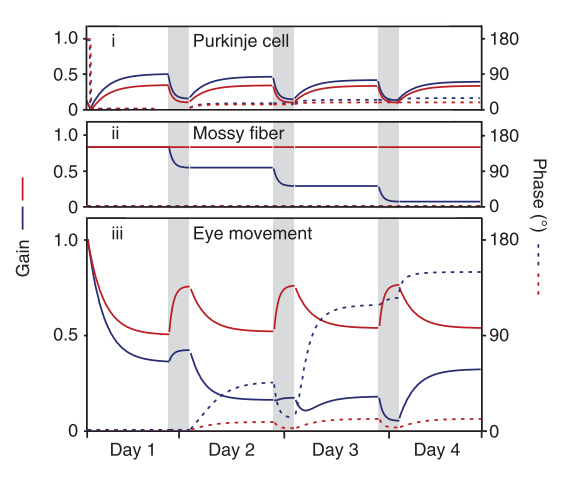
\includegraphics{images/gain.png}

(Wulff et al. 2009)

\end{frame}

\begin{frame}{Reproduction of the results}

Evolution of the gain of the VOR on the different training sessions

(Clopath et al. 2014)

\begin{columns}[T]
\begin{column}[T]{5cm}
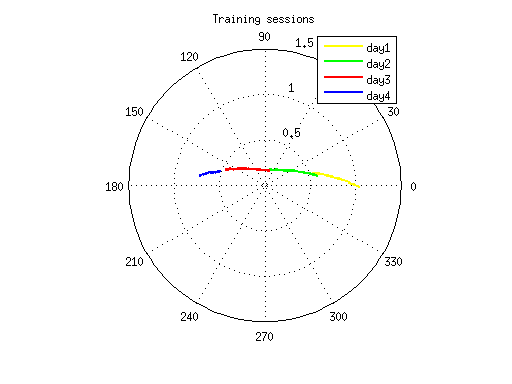
\includegraphics[height=3cm]{images/report_03.png}
\end{column}
\begin{column}[T]{5cm}
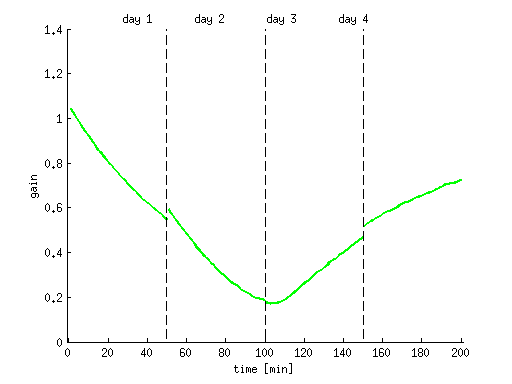
\includegraphics[height=3cm]{images/report_06.png}
\end{column}
\end{columns}

\end{frame}

\begin{frame}{Adding the NOI to the detailed mode}

Modulation in the dark of the teaching signal

\begin{itemize}
\item
  Modulated by vestibular information (Clopath et al. 2014)
  \[C(t) = \nu_{CF} - L(V(t- \delta) - V_t(t-\delta)) - H(M(t) - M_0)\]
\item
  Modulated by cortical information
  \[C(t) = \nu_{CF} - L(V(t- \delta) - V_t(t-\delta)) - H(kP(t))\]
\end{itemize}

\end{frame}

\begin{frame}{Preliminary results}

Evolution of the gain of the VOR on the different training sessions
(arbitrary \emph{k})

\begin{columns}[T]
\begin{column}[T]{5cm}
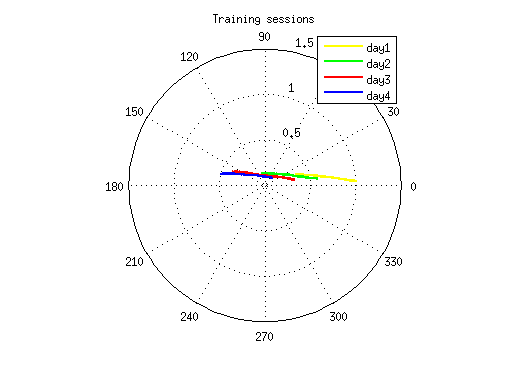
\includegraphics[height=3cm]{images/report_11.png}
\end{column}
\begin{column}[T]{5cm}
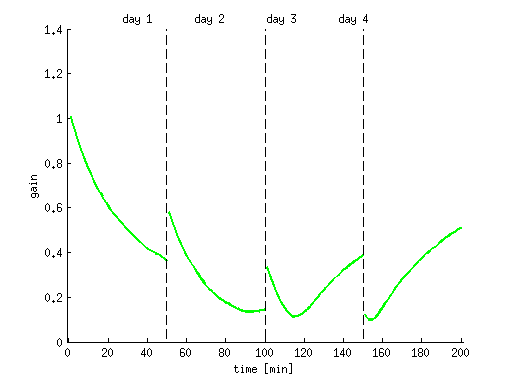
\includegraphics[height=3cm]{images/report_14.png}
\end{column}
\end{columns}

\end{frame}

\begin{frame}{Project planning}

\begin{itemize}
\itemsep1pt\parskip0pt\parsep0pt
\item
  10/2014 to 02/2015: State of the art review
\item
  10/2014 to 11/2014: Implement Clopath's minimal model
\item
  11/2014 to 12/2014: Implement Clopath's detailed model
\item
  12/2014 to 02/2015: Reproducing experimental results
\item
  02/2015 to 03/2015: Add NOI to the model
\item
  03/2015 to 04/2015: Validating the model
\item
  04/2015 to 05/2015: Analyze results
\item
  03/2015 to 06/2015: Writing the report
\end{itemize}

\end{frame}

\begin{frame}{Future work}

\begin{itemize}
\itemsep1pt\parskip0pt\parsep0pt
\item
  Analyze detailed model assumptions

  \begin{itemize}
  \itemsep1pt\parskip0pt\parsep0pt
  \item
    What are the effects of clipping weights on the PF-PC synapses?
  \item
    Identify other assumptions of the detailed model
  \end{itemize}
\item
  Comparing detailed and NOI models

  \begin{itemize}
  \itemsep1pt\parskip0pt\parsep0pt
  \item
    Do they show linear or exponential decay after one week light
    deprivation?
  \item
    What does maintaining the training to the cortex-nuclei memory
    balance?
  \end{itemize}
\end{itemize}

\end{frame}

\begin{frame}{References}

\fontsize{6}{10} \selectfont

Brandi, Santiago, Ivan Herreros, and Paul F M J Verschure. 2014.
``Optimization of the Anticipatory Reflexes of a Computational Model of
the Cerebellum,'' no. 1: 11--22.

Clopath, Claudia, Aleksandra Badura, Chris I {De Zeeuw}, and Nicolas
Brunel. 2014. ``A Cerebellar Learning Model of Vestibulo-Ocular Reflex
Adaptation in Wild-Type and Mutant Mice.'' \emph{J. Neurosci.} 34 (21):
7203--15.
doi:\href{http://dx.doi.org/10.1523/JNEUROSCI.2791-13.2014}{10.1523/JNEUROSCI.2791-13.2014}.
\url{http://www.ncbi.nlm.nih.gov/pubmed/24849355}.

Herreros, Ivan, and Paul F M J Verschure. 2013. ``Nucleo-Olivary
Inhibition Balances the Interaction Between the Reactive and Adaptive
Layers in Motor Control.'' \emph{Neural Netw.} 47 (November). Elsevier
Ltd: 64--71.
doi:\href{http://dx.doi.org/10.1016/j.neunet.2013.01.026}{10.1016/j.neunet.2013.01.026}.
\url{http://www.ncbi.nlm.nih.gov/pubmed/23535576}.

Ito, Masao. 2006. ``Cerebellar Circuitry as a Neuronal Machine.''
\emph{Prog. Neurobiol.} 78 (3-5): 272--303.
doi:\href{http://dx.doi.org/10.1016/j.pneurobio.2006.02.006}{10.1016/j.pneurobio.2006.02.006}.
\url{http://www.ncbi.nlm.nih.gov/pubmed/16759785}.

Ke, Michael C, Cong C Guo, and Jennifer L Raymond. 2009. ``Elimination
of Climbing Fiber Instructive Signals During Motor Learning.''
\emph{Nat. Neurosci.} 12 (9). Nature Publishing Group: 1171--9.
doi:\href{http://dx.doi.org/10.1038/nn.2366}{10.1038/nn.2366}.
\url{http://www.pubmedcentral.nih.gov/articlerender.fcgi?artid=3864777/\&tool=pmcentrez/\&rendertype=abstract}.

Wulff, Peer, Martijn Schonewille, Massimiliano Renzi, Laura Viltono,
Marco Sassoè-Pognetto, Aleksandra Badura, Zhenyu Gao, et al. 2009.
``Synaptic Inhibition of Purkinje Cells Mediates Consolidation of
Vestibulo-Cerebellar Motor Learning.'' \emph{Nat. Neurosci.} 12 (8):
1042--9. doi:\href{http://dx.doi.org/10.1038/nn.2348}{10.1038/nn.2348}.
\url{http://www.pubmedcentral.nih.gov/articlerender.fcgi?artid=2718327/\&tool=pmcentrez/\&rendertype=abstract}.

\end{frame}

\end{document}
